In the last years, the computer science world is witnessing the rise of the \textit{big data} era. In fact world population is  increasing continuously and, as shown in \cite{World} at the beginning of January 2016 there were 7,392 billions of people. As the population grow, also data produced by people grow (thanks to the contemporary diffusion of technologies).
According to an article published on Teradata Magazine in 2011 we can say that:
\begin{quote}
"Big data exceeds the reach of commonly used hardware environments and software tools to capture, manage, and process it with in a tolerable elapsed time for its user population."
\end{quote}
The next part of this chapter will show the importance of these data in the modern world and the new challenges they offer.

\section{Importance and value of data}\label{sec12:DataValues}
As we can see in \cite{EMC1}, the digital universe is doubling in size every two years and by 2020 it will contain as many digital bits as the stars in the universe (about 44 zettabytes). These data come from a huge number of different sources like tweets, videos, sensors, etc..., and their union is important for modern systems (as in the \textit{internet of things}).
These data are defined and can be processed by software, for extraction of the various informations. Companies that will be able to master big data will gain an enormous economical power. Kaggle CEO Anthony John Goldbloom, says: 
\begin{quotation}
"The bigger the data set you have, the more accurate the predictions about the future will be"
\end{quotation}
This means that our predictive systems work better when they have a lot of data to examine and this is the main reason for dealing with big data. In addition, from a scientific point of view, accurate experiments require a big amount of data to work on. An example is given by \textit{Google Translate}. The popular translation service use collections of snippets of translations which are continuously debugged by users. It works fine because Google has tons of snippets from the indexed web pages, and the accuracy of the service improves as the training set grows.\\

Summing up the characteristics we have already seen, IBM data scientists break big data into four dimensions:
\begin{itemize}
 \item \textbf{Volume}: big data volumes are typical in the order of Terabytes and are growing year by year
 \item \textbf{Variety}: big data come from a huge number of sources
 \item \textbf{Velocity}: speed in streaming data processing is essential, otherwise we will be overwhelmed by these big volumes. For example modern cars have about 100 sensors, so we need to be fast to process their informations to make the correct decision about driving. Another example come from finance world, in fact the New York Stock Exchange, captures 1 Terabyte of trading information that needs to be fast processed to make the right decision in the lesser time possible.
 \item \textbf{Veracity}: as already said we need big data to produce better predictions from our analysis systems. However, we need to have the best data possible in order to predict as \textit{accurate} as possible. This dimension is so important that IBM data scientists said that poor data quality costs the US economy around 3.1 trillions of dollars a year
\end{itemize}

\begin{figure}[htb] %  figure placement: here, top, bottom
   \centering
   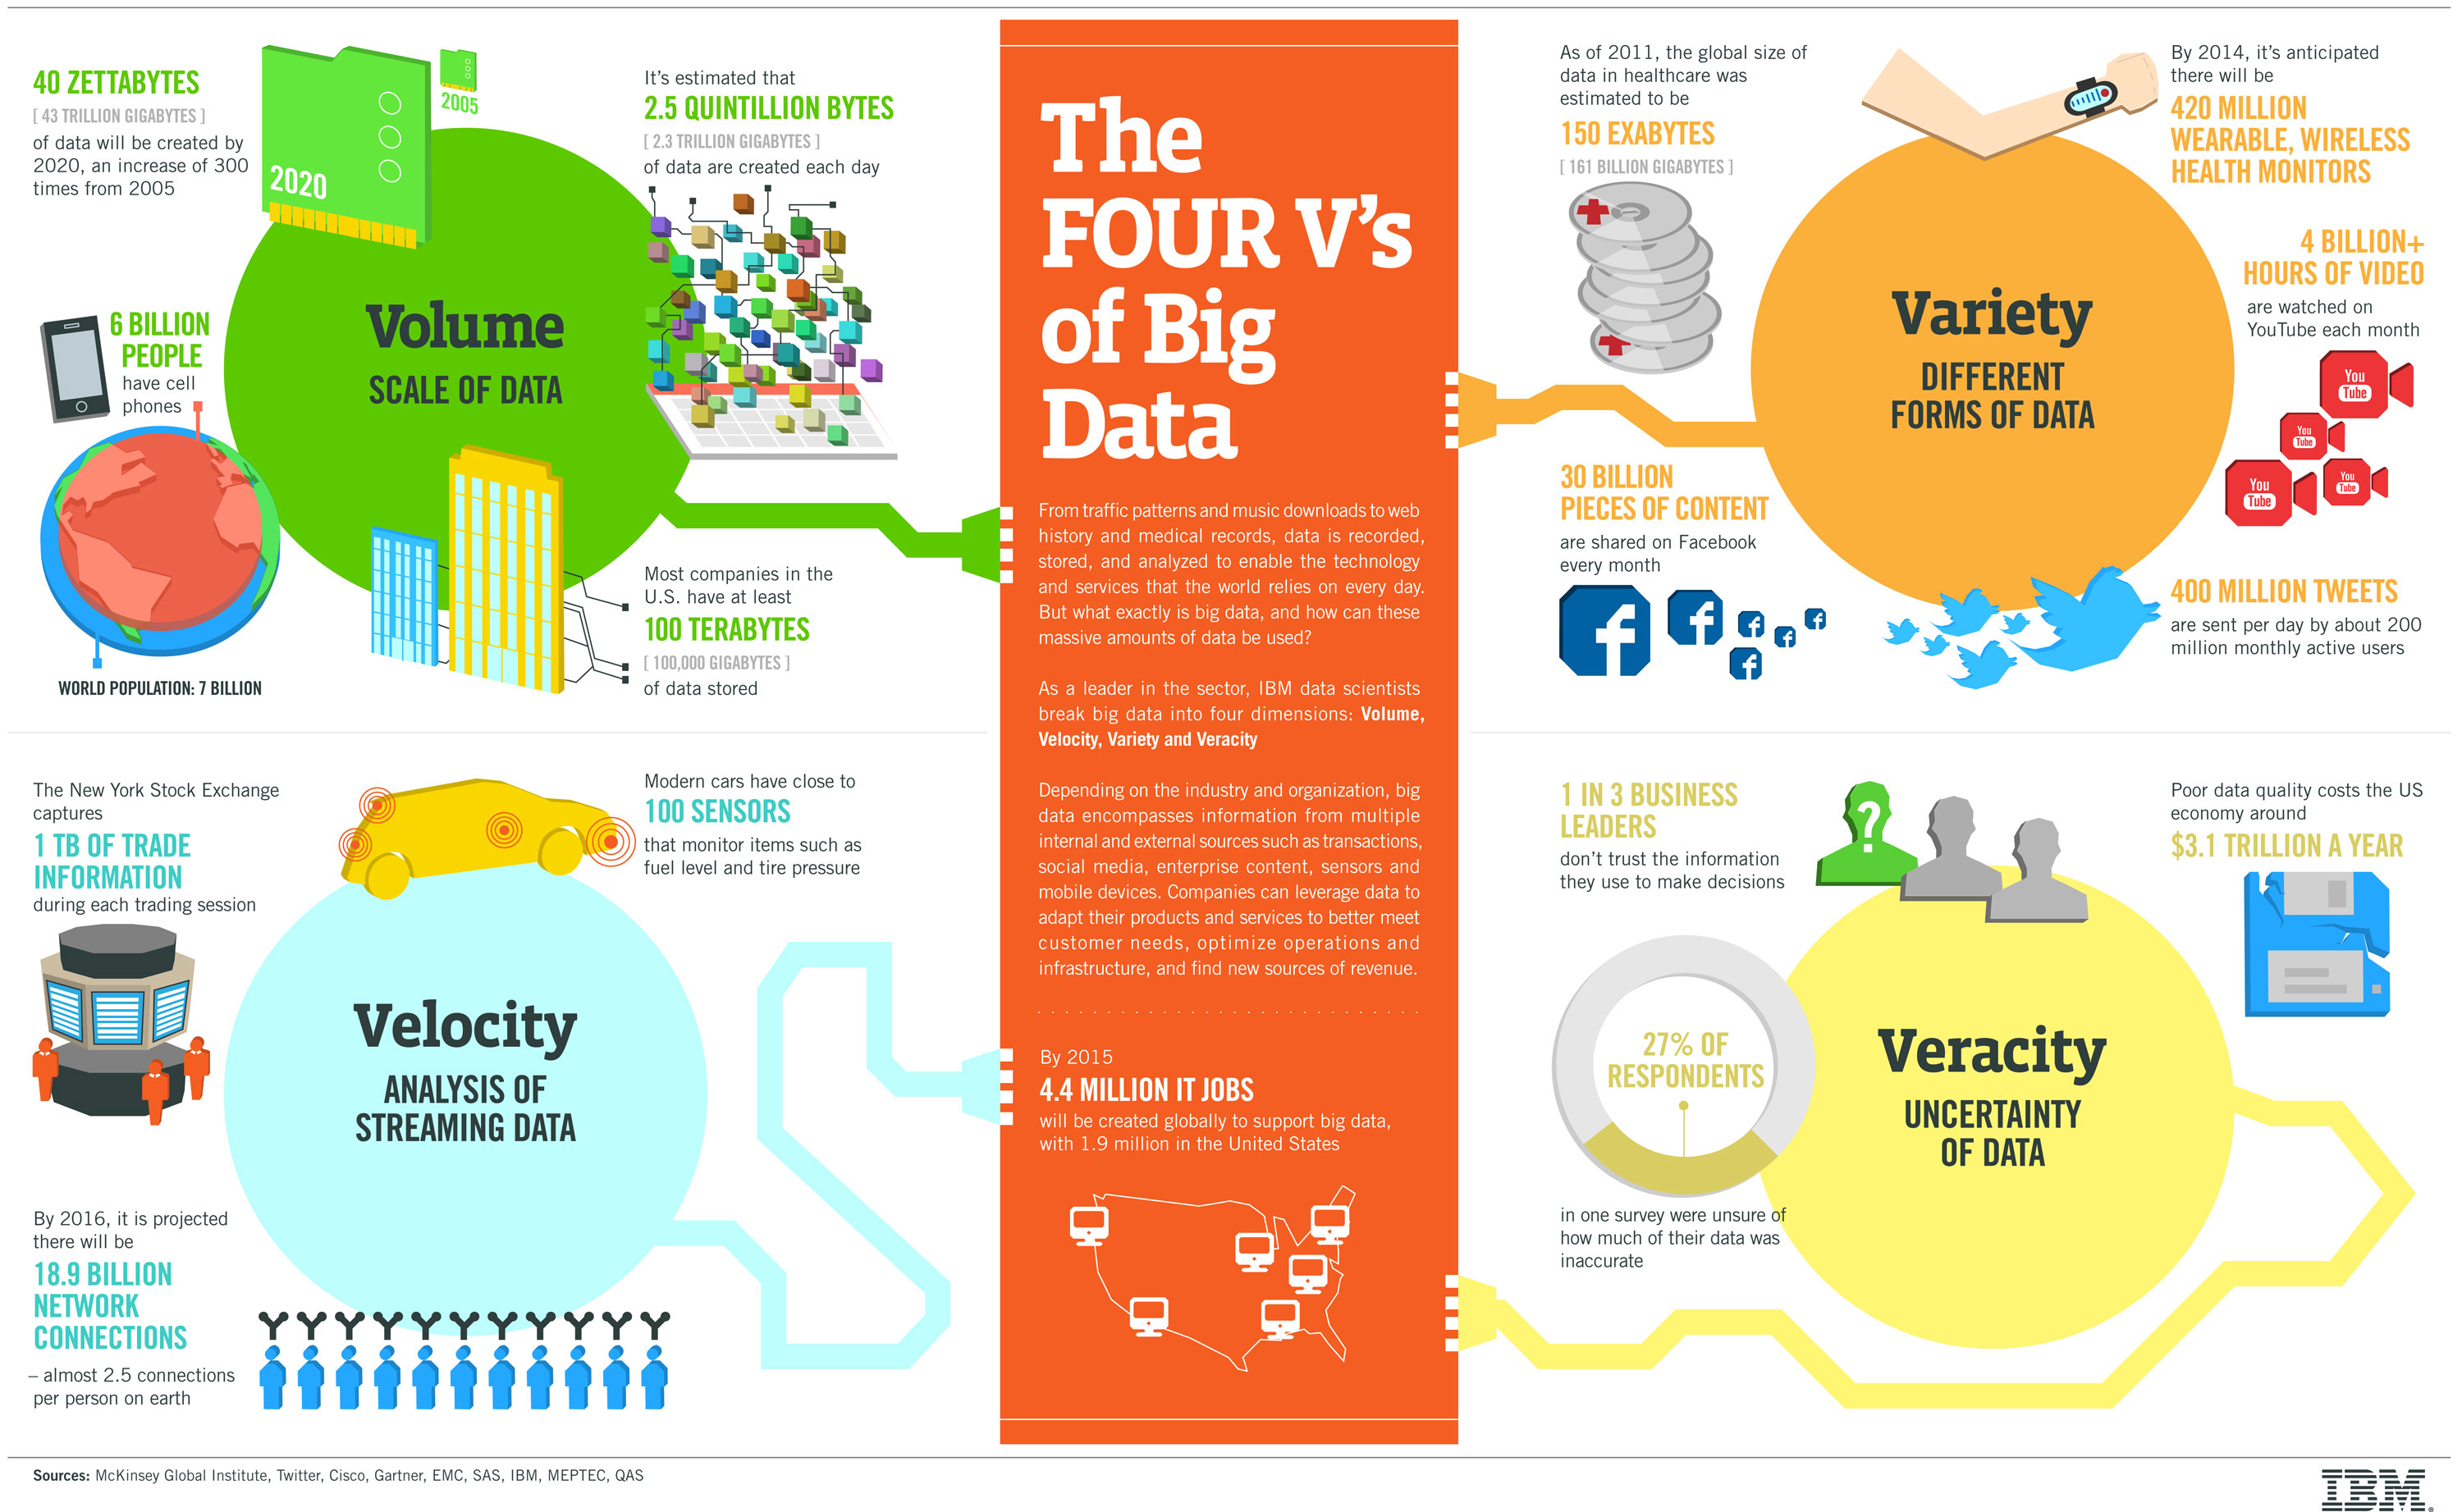
\includegraphics[width=1.0\linewidth]{images/4-Vs-of-big-data.jpg}\hfill
   \caption[The four V of big data]{The four V of big data according to an infographic distributed by IBM data scientists}
   \label{fig:fourV}
\end{figure}

\section{Typical problems when dealing with big data}\label{sec12:bigDataProblems}

In the earlier section, we have read about the advantages of big data. However, as shown in \cite{EMC1}, the digital universe may actually be an obstacle for companies trying to become data-driven. There is too much information, it is too diverse, and it is too effervescent. Summing up we can say that:
\begin{itemize}
 \item there is more heterogeneity
 \item data grows faster than energy in chip
 \item we still need humans to ask right questions for information extraction
\end{itemize}

These problems sometimes lead to wrong results from big data analysis.
For example as pointed out in \cite{Lazer}, \textit{Google Flu Trends} service (which provides estimates of influenza activity by aggregating Google search queries), overestimated flu prevalence (sometimes it predicted twice as many doctors' visits). One of the problems was that people making searches about flu, knew very little about how to diagnose it. So searches for flu or flu symptoms may regard diseases that are similar to flu but are not. Moreover changes in Google search algorithm over time, have raised concerns about the meaning of its predictions.\\

Another problem with big data is output misunderstanding. In fact after we have applied an analysis method on our big data, we have to be sure about conclusions; sometimes we could find strange correlations, unexpected results (like Google Flu Trends) or we risk to bad interpret the data.\\

We can also have technical problems when dealing with big data. They substantially regard computation speed and \textbf{memory consumption}. In particular the latter is the worst one, because we could tolerate waste of time in a lot of applications, but we cannot tolerate an algorithm that does not work when input grow too much. A common solution to these problems consists in \textit{scale out} our architectures distributing the algorithm as we will see in Chapter~\ref{Chapter22}. Another solution consist in choosing a better analysis technique. As we have already seen in Chapter~\ref{Chapter11}, human vision has a great ability to synthesize big data. For this reason scientific visualization can represent a great help for these problems and in the following parts of this work we will see how it can be useful in medical research

\section{Big data collections and big data objects}\label{sec12:bigDataCollectionsObjects}

Now we will consider some issues in managing big data in the scientific visualization field. As we can see in \cite{Cox}, this is an old problem (the paper was published in 1997), nowadays still to be solved. According to this paper problems with big data come from:
\begin{itemize}
 \item \textbf{Big data collections}
 \item \textbf{Big data objects}
\end{itemize}

Big data collections are aggregates of many datasets. The size of data may typically exceed the capacity of storage (usually disks), so it can be partitioned between several storage devices. Generally speaking, big data collections present the following problems:
\begin{itemize}
 \item Data are distributed among multiple sites
 \item Data reside in heterogeneous databases
 \item Data are generally not self-describing
 \item Often they do not have meta-data
 \item There may be poor data locality for the queries
 \item Data access time may be quite high due to partitioning
\end{itemize}

Instead, big data objects typically comes from large-scale simulations and are usually multi-dimensional datasets. For example in computational fluid dynamics, a common data structure is a set of curvilinear grids with computed values at the vertices of the grids.\\
Data objects, typically present the following problems:
\begin{itemize}
 \item Multi-dimensional data structures are not adequately supported by database technology
 \item A single data object may not fit in the main memory or, in the worst case, it may be too big for local disks
 \item Latencies and bandwidths between the data store and main memory must be managed carefully
\end{itemize}

Obviously we can also have the combined problem: \textit{big collections of big objects}.\\

Now we have understood the main problems that arise when dealing with big data especially in scientific visualization field. This knowledge will help us further on as we will learn of the methodologies for mastering big data complexity. In particular, we will see how to \textit{scale out} our architectures using parallel programming, solving all problems regarding the volume of the data
